\documentclass{pgnotes}

\title{Power}

\begin{document}

\maketitle

\section{Electrical basics}

\autoref{tab:key-electrical-quantities} summarises key electrical quantities.

\begin{table}[htbp]
  \centering
  \begin{tabular}{l l l l}
    \toprule
    \textbf{Quantity} & \textbf{Symbol} & \textbf{Unit} & ~ \\
    \midrule
    Voltage & $V$ & Volt & \si{\volt} \\
    Current & $I$ & Ampere & \si{\ampere} \\
    Resistance & $R$ & Ohm & \si{\ohm} \\
    Power & $P$ & Watt & \si{\watt} \\
    \bottomrule
  \end{tabular}
  \caption{Key electrical quanities}
  \label{tab:key-electrical-quantities}
\end{table}

Note that voltage is a difference between \textit{two} points.
Often measured in any system with respect to a common earth / ground.

\subsection{Ohm's law}
  
Voltage, current and resistance are related by Ohm's law, which can be written in terms of $V$, $I$ or $R$.
Re-arrange to calculate required quantity.
\begin{align}
  V & = R \cdot I \\
  \Rightarrow I & = \frac{V}{R} \\
  \Rightarrow R & = \frac{V}{I}      
\end{align}

\begin{example}{Ohm's law}{ohms-law-v}
  A \SI{7}{\ohm} resistance carries a current of \SI{2}{\ampere}.
  Determine the voltage across the component.
  \tcblower
  \begin{align}
    V & = 7 \times 2 \\
      & = \SI{14}{\volt}
  \end{align}
\end{example}

\begin{example}{Ohm's law with rearrangement}{ohms-law-r}
  When an electrical component is connected across a battery nominally supplying \SI{12}{\volt} a current of \SI{3}{\ampere} flows.
  Calculate the resistance of the component.
  \tcblower
  \begin{align}
    V & = R \cdot I \\
    \Rightarrow R & = \frac{V}{I} \\
      & = \frac{12}{3} \\
      & = \SI{4}{\ohm}
  \end{align}
\end{example}

\subsection{Power}

Power quantifies how much energy is converted from one form to another per unit time. Measured in Joule per second \si{\joule\per\second}, more commonly the Watt \si{\watt}.
Just as with Ohm's law, the power relation, \autoref{eq:power-P}, can be rearranged to give $V$ or $I$:
\begin{align}
  P & = V \cdot I \label{eq:power-P} \\
  \Rightarrow V & = \frac{P}{I} \label{eq:power-V} \\
  \Rightarrow I & = \frac{P}{V} \label{eq:power-I} 
\end{align}

\begin{example}{Power calculation}{power-V}
  A graphics card is supplied from the \SI{12}{\volt} power supply in a computer. The current flowing is measured at \SI{5}{\ampere}. Determine the power consumed by the graphics card.
  \tcblower
  \begin{align}
    P & = 12 \times 5 \\
      & = \SI{60}{\watt} 
  \end{align}
\end{example}

\begin{example}{Power calculation with rearrangement}{power-I}
  A computer power supply delivers \SI{6}{\watt} to a hard disk drive on the \SI{12}{\volt} line.
  Determine the current flowing in the cable.
  \tcblower
  \begin{align}
     I & = \frac{P}{V} = \frac{6}{12} \\
      & = \SI{0.5}{\ampere}
  \end{align}
\end{example}




\section{Mains electricity}

In Ireland, mains electricity is supplied at a \textit{nominal} \SI{230}{\volt} \SI{50}{\hertz}.
Mains wiring in Ireland generally involves three conductors:
\begin{description}
\item[Live (or hot, or phase)] carries a \SI{230}{\volt} RMS AC voltage.
\item[Neutral] provides the return path for current on the live conductor, and under normal conditions will be the negative of that.
\item[Earth] is connected to earth and bonded to metal casings.
\end{description}


\subsection{Circuit protection}

\begin{description}
\item[Fuses:] a piece of thin wire encased in a holder that is deliberatly designed to melt if the current exceeds the fuse rating.
\item[Circuit Breakers (MCB):] electromechanical devices that will trip when the current exceeds the circuit breaker's rating.
\item[Residual current device (RCD):] protect from electric shock by detecting any leakage of current to earth by comparing live and neutral currents.
  Trips if these differ by more than a set amount $\Delta I$, normally \SI{30}{\milli\ampere}.
  Other names: GFI, ELCB.
\item[Residual Current Breaker Overload (RCBO):] combined MCB and RCD functionality in one device.
\end{description}


\subsection{Alternating current (AC)}

Mains electricity is supplied in most parts of the world as alternating current (AC).
This means that the instantaneous voltage $v(t)$ varies sinusoidally with respect to time.
\begin{align}
  v(t) & = V_{\mbox{max}} \sin ( 2 \pi f t ) \label{eq:ac-instantaneous-voltage}
\end{align}
A single cycle of a generic AC waveform is shown in \autoref{fig:ac-waveform-properties}

\autoimage{ac_waveform_properties}{AC waveform properties}{ac-waveform-properties}

The \textbf{maximum voltage} $V_{\mbox{max}}$ of a sinusoid is the amplitude of the sine wave in both directions.
The most positive value is $V_{\mbox{max}}$ whilst the most negative value is $-V_{\mbox{max}}$.
We can thus define the \textbf{peak-to-peak} amplitude as the difference between these two values:
\begin{align}
  V_{\mbox{PK-PK}} & = V_{\mbox{max}} - ( - V_{\mbox{max}} ) \\
                   & = 2 V_{\mbox{max}}                    
\end{align}

\begin{example}{Peak-to-peak to amplitude}{pkpk-amplitude}
  Calculate the amplitude of an AC waveform with a \SI{650}{\volt} peak-to-peak amplitude.
  \tcblower
  \begin{align}
    V_{\mbox{max}} & = \frac{V_{\mbox{PK-PK}}}{2} \\
                   & = \frac{650}{2} \\
                   & = \SI{325}{\volt} 
  \end{align}
\end{example}

\subsubsection{RMS Voltage}

The voltage in western Europe is a nominal \SI{230}{\volt}~RMS.
This is a root mean square value, which is equivalent to the heating power that the same DC voltage would deliver.
\begin{align}
  V_{\mbox{max}} & = \sqrt{2} V_{\mbox{RMS}} \\
  \Rightarrow V_{\mbox{RMS}} & = \frac{V_{\mbox{max}}}{\sqrt{2}}
\end{align}

\begin{example}{RMS to peak voltage}{rms-to-peak-voltage}
  Calculate the amplitude of a \SI{230}{\volt} RMS AC supply.
  \tcblower
  \begin{align}
    V_{\mbox{max}} & = \sqrt{2} V_{\mbox{RMS}} \\
                   & = \sqrt{2} \times 230 \\
                   & = \SI{325}{\volt}                    
  \end{align}
\end{example}

\begin{example}{Peak to RMS voltage}{peak-to-rms-voltage}
  Calculate the RMS voltage of an AC supply with an amplitude of \SI{100}{\volt}.
  \tcblower
  \begin{align}
    V_{\mbox{RMS}} & = \frac{V_{\mbox{max}}}{\sqrt{2}} \\
                   & = \frac{100}{\sqrt{2}} \\
                   & = \SI{70.7}{\volt} 
  \end{align}
\end{example}

\subsubsection{Frequency / Period}
A single cycle lasts for a period of time, $T$.
The period is directly related to the frequency:
\begin{align}
  T & = \frac{1}{f} \\
      \Rightarrow f & = \frac{1}{T}
\end{align}
\begin{example}{Frequency to period}{frequency-to-period}
  Calculate the period of a signal that repeats at \SI{20}{\hertz}.
  \tcblower
  \begin{align}
    T & = \frac{1}{20} \\
      & = \SI{0.05}{\second} 
  \end{align}
\end{example}
\begin{example}{Period to frequency}{period-to-frequency}
  Determine the frequency of a signal with a period of \SI{40}{\milli\second}.
  \tcblower
  \begin{align}
    f & = \frac{1}{\num{40e-3}} \\
      & = \SI{25}{\hertz}
  \end{align}
\end{example}


% \begin{exercise}{Mains electricity}{mains-electricity}
%   \begin{enumerate}
%   \item The AC mains supply in Ireland has a frequency of \SI{50}{\hertz}. Calculate the period of the AC waveform.
%   \item Trains in parts of Europe are supplied with \SI{15}{\kilo\volt} AC at 16 \SI[quotient-mode=fraction]{2/3}{\hertz}. How often does the AC cycle repeat?
%   \item An unknown mains supply is measured to be sinusoidal with an amplitude of \SI{339.4}{\volt} and a frequency of \SI{50}{\hertz}. Describe this supply in the conventional form.
%   \end{enumerate}
% \end{exercise}

\section{Computer power supplies}

Power Supply Units (PSUs) are used to convert the mains-supplied power into a form suitable for use in computers.

\subsection{Computer power requirements}

Computers require a variety of DC voltages, the most common being:
\begin{description}
\item[\SI{3.3}{\volt}] (orange)
\item[\SI{5}{\volt}] (red)
\item[\SI{12}{\volt}] (yellow).
\end{description}
These are normally supplied relative to a common ground (black).
\begin{description}
\item[Negative \SI{-12}{\volt}] (blue) is often available.
\end{description}
A PSU also permanently supplies \SI{5}{\volt} (purple) and will turn on when the green terminal is shorted to ground.

\subsection{Power supply tasks}

A computer's power supply unit (PSU) has two key jobs:
\begin{description}
\item[Rectify] the mains-supplied AC to a steady DC supply.
\item[Step down] the voltage (\SI{230}{\volt}) to the required level(s).
\end{description}
The precise methods and order that these tasks are performed in will vary, and are outside the scope of our discussion.

\subsection{Capacity}

A power supply will usually have a rated capacity:
\begin{itemize}
\item This will either be given in terms of power (watts) or in current (amps).
\item On a supply providing multiple voltages, there will usually be a limit on each rail as well as possibly an overall limit.
\end{itemize}

\subsection{Three-phase supply}

Mains power is generated and distributed in three-phase form, with 3 live conductors and one neutral conductor.
The sine wave is shifted by 120 degrees, or $\frac{2\pi}{3}$ radians in any phase relative to one of the two other phases.

\autoimage{3_phase_waveform}{3-phase waveform (Wikipedia)}{3-phase-waveform}

Let $v_n(t)$ be the voltage in phase $n$ of a three-phase supply.
We can use \autoref{eq:ac-instantaneous-voltage} for the first phase.
Phase~2 must lags phase 1 by 120 degrees.
Similarly, phase~3 leads phase~1 by 120 degrees.
\begin{align}
  v_1(t) & = V_{\mbox{max}} \sin ( 2 \pi f t ) \\
  v_2(t) & = V_{\mbox{max}} \sin \left ( 2 \pi f t - \frac{2\pi}{3} \right ) \\
  v_3(t) & = V_{\mbox{max}} \sin \left ( 2 \pi f t + \frac{2\pi}{3} \right )                      
\end{align}

\subsubsection{Line and phase voltages}

When dealing with three-phase power, we actually have two voltages to consider:
\begin{description}
\item[Phase voltage] is the voltage between \textit{any} phase and neutral.
\item[Line voltage] is the voltage measured between \textit{any} two phases.
\end{description}

The line and phase voltages are related mathematically by $\sqrt{3}$:
\begin{align}
  V_{\mbox{line}} & = \sqrt{3} \times V_{\mbox{phase}}\\
\Rightarrow  V_{\mbox{phase}} & = \frac{V_{\mbox{line}}}{\sqrt{3}}                     
\end{align}

\begin{example}{Line to phase voltage}{line-to-phase-voltage}
  A three phase power supply has a phase voltage of \SI{220}{\volt}.
  Calculate the line voltage.
  \tcblower
  \begin{align}
    V_{\mbox{line}} & = \sqrt{3} \times V_{\mbox{phase}} \\
                     & = \sqrt{3} \times 220  \\
                     & = \SI{381}{\volt}
  \end{align}
\end{example}

\begin{example}{Phase to line voltage}{phase-to-line-voltage}
  A three phase power supply has a line voltage of \SI{400}{\volt}.
  Calculate the phase voltage.
  \tcblower
  \begin{align}
    V_{\mbox{phase}} & = \frac{V_{\mbox{line}}}{\sqrt{3}} \\
                     & = \frac{400}{\sqrt{3}} \\
                     & = \SI{231}{\volt}
  \end{align}
\end{example}

\newpage
\section{Distribution path}

\autoref{fig:power-distribution} shows the basic power distribution hierarchy in a data centre.

\begin{figure}[htbp]
  \centering
  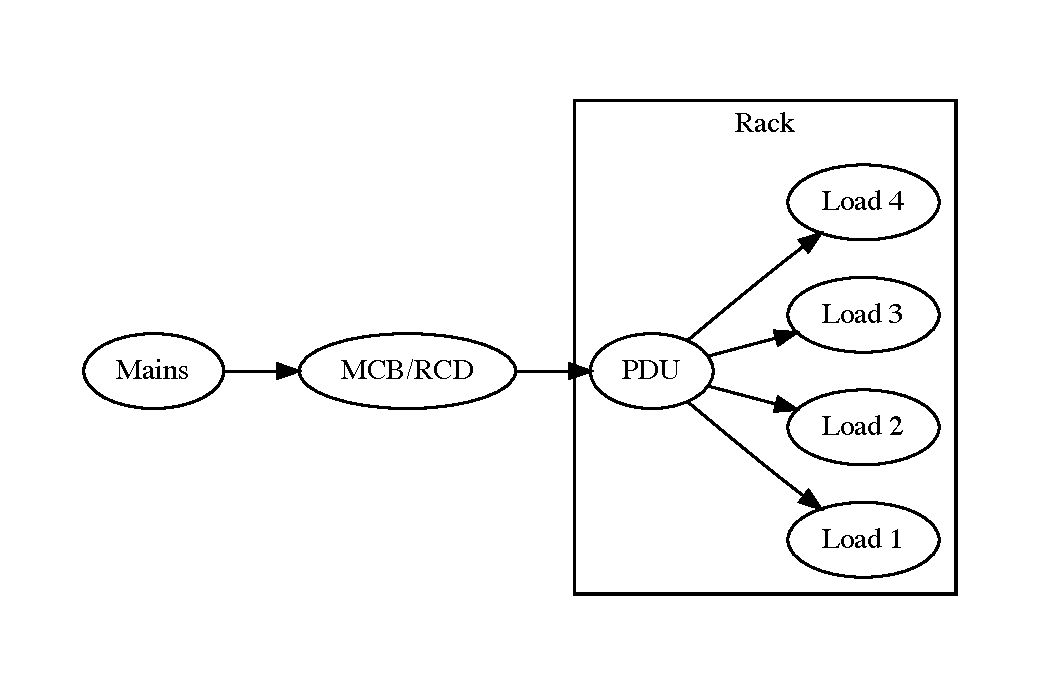
\includegraphics[width=0.5\linewidth]{power_distribution_diagram}
  \caption{Power distribution schematic}
  \label{fig:power-distribution}
\end{figure}

We will consider the distribution path looking \textit{backwards} from the IT equipment towards the incoming mains.


\subsection{Power distribution unit (PDU)}

Each rack normally has a power distribution unit, which is no more complicated than a multiplug adapter:
\begin{itemize}
\item PDU can be mounted vertically in the back of rack or in a rack space (facing in or out).
\item PDUs are available with various combinations of input and output connectors.
\item PDUs may or may not have surge protection and switches.
\item Maximum current will usually be dependent on the connector type on the input to the PDU.
\item ``Smart'' PDUs are available that can measure power demand and turn on/off sockets remotely. (See later on!)
\end{itemize}

\subsection{Common connectors}

\autoref{tab:common-mains-plugs-sockets} shows the most common mains power connectors (plugs and sockets) that will be encountered in a data centre environment.

\begin{table}[htbp]
  \centering  
  \begin{tabular}{l r r r}
    \toprule
    \textbf{Type} & $I_{\mbox{max}}$ & \textbf{Male} & \textbf{Female} \\
    \midrule
    BS~1363 & \SI{13}{\ampere} & ~ & ~ \\
    \midrule
    IEC~C13/14 & \SI{10}{\ampere} & C14 & C13 \\
    \midrule  
    IEC~C19/20 & \SI{16}{\ampere} & C20 & C19 \\
    \midrule  
    IEC~60309 & \SI{16}{\ampere} & ~ & ~ \\
    \bottomrule
  \end{tabular}
  \caption{Common connector types}
  \label{tab:common-mains-plugs-sockets}
\end{table}


\section{Disturbances}

Our IT equipment expects clean power with its key parameters (voltage, frequency) maintained within allowable tolerences (\SI{230}{\volt} RMS, \SI{50}{\hertz}).
Waveform must be a \textit{clean} sine wave, not \textit{distorted}.

\subsection{Disturbance types}

\begin{description}
\item[Blackout:] total loss of power.
\item[Surge/sag:] \textbf{short-term} (0.5 of a cycle up to 1 minute) voltage variations:
\begin{description}
\item[Surge or spike] is a short-term high-voltage condition more than \SI{110}{\percent} of the nominal value.
\item[Sag] is a short-term low-voltage condition.
\end{description}

\item[Over and under-voltage] conditions that \textbf{persist for time periods} ranging from minutes to days:
\begin{description}
\item[Over-voltage] is increased mains voltage.
\item[Under-voltage] is reduced mains voltage.  (Formerly: brownout)
\end{description}

\item[Frequency fluctuations] away from \SI{50}{\hertz} for long and short periods.

\item[Waveform distortion] when the mains voltage waveform no longer is a sinusoid.
This can manifest in a number of ways: offsets, harmonics, notching and noise.

\end{description}

\newpage

\subsection{CBEMA curve}

Undesirable conditions are generally less disruptive the shorter that they persist for.
This includes disturbances in the power supply.
The Computer Business Equipment Manufacturers Association (CBEMA) in the 1970s generated a curve that partitioned voltage events and times into acceptable and unacceptable region.
The Information Technology Industry Council (ITIC) adapted the curve in the 1990s, which was most recently updated in 2000, \autoref{fig:itic-cbema-curve}

\begin{figure}[htbp]
  \centering
  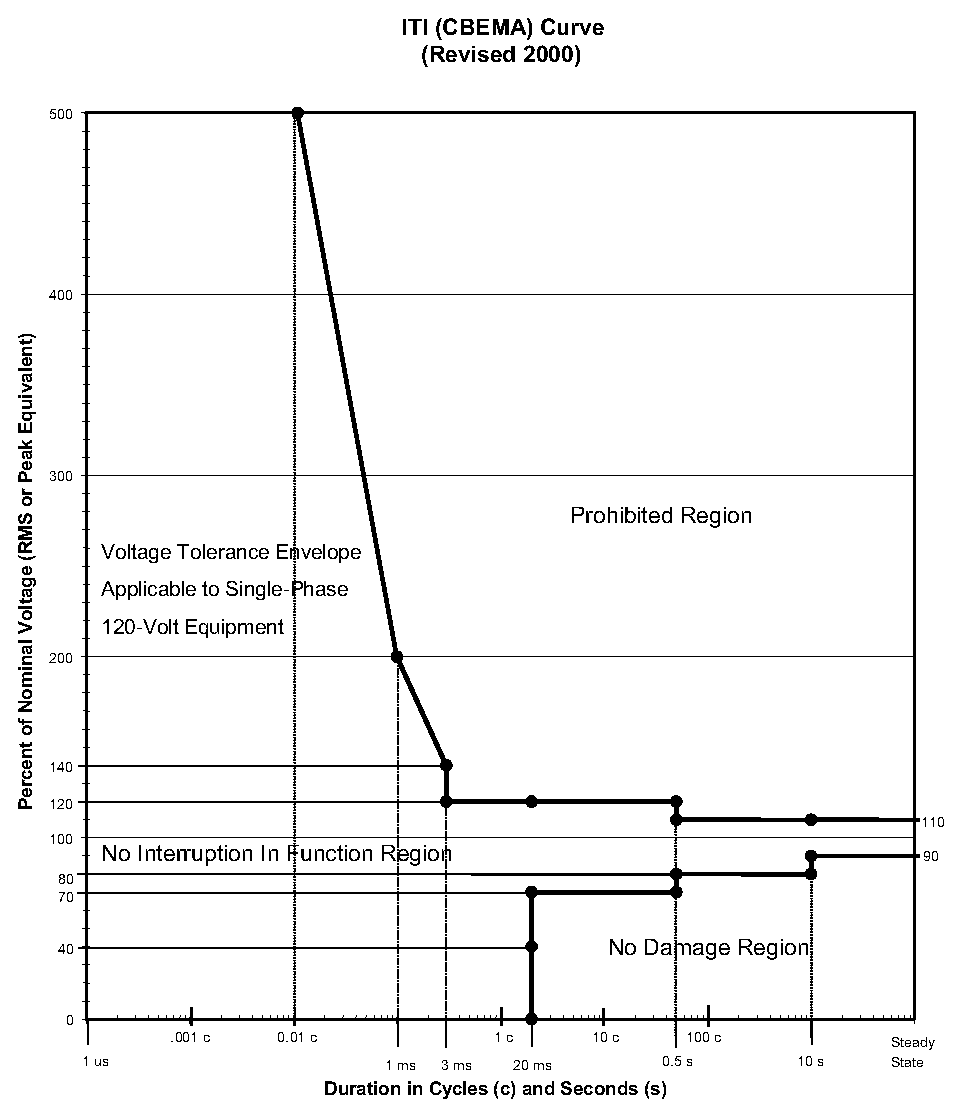
\includegraphics[width=0.9\linewidth]{iti_cbema_curve}
  \caption{ITI CBEMA Curve 2000}
  \label{fig:itic-cbema-curve}
\end{figure}

\newpage

\section{Uninterruptible Power Supplies (UPS)}

\subsection{Key Components}
UPS units are complex devices but contain a number of key building blocks you should know: 
\begin{description}
\item[Battery] as an energy storage medium.
  Common types include: Lead-Acid, Nickel-Cadmium (NiCd), Nickel Metal Hydride (NiMH), Lithium-Ion. 
\item[Rectifier] to convert mains AC to DC for battery charging.
\item[Inverter] to take DC and convert it to AC at a given voltage and frequency.
\item[Transfer switch] to swap between two sources of power. Can be a mechanical relay or contactor\footnote{A contactor is the conventional name used for a large relay able to switch many amperes of current.} but is more usually solid-state, called a \textit{static transfer switch} or STS.
\item[Surge suppressor:] a solid-state device that reduces voltage by letting current flow to earth when a voltage exceeds the so-called \textit{let through} voltage.
\end{description}


\subsection{Form factors}

UPS units are available in various form factors:
\begin{description}
\item[Freestanding / tower] similar to PC powering a single device or multiple devices via a PDU.  Usually located adjacent to the IT equipment.
\item[Rackmount] powering a single device or multiple devices via a PDU. Usually co-located inside the same rack as the IT equipment.
\item[Floor-standing] UPS devices located within the IT environment itself or in another part of the facility. These normally supply multiple IT loads and are often managed by facilities rather than IT personnel. 
\end{description}


\newpage
\subsection{UPS types}

There are three main categories of UPS: standby, line-interactive and double conversion. 
%For a thorough treatment of the different types of UPS systems see \citet{rasmussen:2011:the-different}.
All UPS devices will protect against blackout (for as long as their batteries last).

\subsubsection{Standby}

A standby UPS normally just passes the utility through to the output, while performing basic surge suppression, \autoref{fig:standby-ups-schematic}.

\autoimage{ups_standby_schematic}{Standby UPS schematic (APC)}{standby-ups-schematic}

The battery is charged from the mains.
Under failure of the mains supply, the UPS will use its inverter to generate AC.
The transfer switch changes the output from utility to inverter.

The standby UPS protects against blackouts and small surges/sags whilst remaining online.
It will transfer to inverter supply in the case of under/over voltage conditions.

\subsubsection{Line interactive}

A line interactive UPS is capable of correcting reasonably small under/over voltage conditions \textbf{whilst remaining online}, \autoref{fig:line-interactive-ups-schematic}.

\autoimage{ups_line_interactive_schematic}{Line interactive UPS schematic (APC)}{line-interactive-ups-schematic}

The line interactive UPS will correct surges/sags and under/over voltage whilst remaining online.
It will use transfer to battery power to correct issues with AC frequency and waveform quality.

\subsubsection{Double conversion}

The double-conversion UPS differs from the standby and line-interactive UPS in that it doesn't differentiate between online/offline modes of operation.
Double conversion UPS units correct both voltage and frequency disturbances.
\autoref{fig:double-conversion-ups-schematic}.

\autoimage{ups_double_conversion_schematic}{Double conversion UPS schematic (APC)}{double-conversion-ups-schematic}

They consist of a battery bank charged by the mains, from which an inverter generates a clean AC waveform at the right voltage and frequency,


\section{UPS sizing}

UPS sizing needs to consider how much power the UPS is expected to supply (determines inverter size), and for how long (determines battery size).
The reactive / apparent power requirements need to be considered. 

Specifying a UPS is a somewhat inexact process.
A undersized unit will not work, but an oversized unit will.
Therefore, we normally pad calculated requirements by a \SI{20}{\percent} buffer.

\subsection{Real power requirements}

The UPS power required, with padding, can be calculated:
\begin{align}
  P_{\mbox{total}} & = \left ( \sum_{\mbox{devices}} P_{\mbox{device}} \right ) \times 1.2
\end{align}


\subsection{Apparent power}

When sizing power distribution components, we need to consider the so-called Volt-Amp rather than the Watt.
So far we know that the watt is the unit of power.
From the power relation we first met in \autoref{eq:power-P}, $P = V \cdot I$, we might reasonably expect that $\SI{1}{\watt}=\SI{1}{\volt\ampere}$.
However, in real life this isn't the case.

\subsubsection{Reactive power}

In simple loads like incandescent lights and heaters, regardless of size, the current and voltage will be perfectly in phase.
However, with many real-world loads the current wave will lead or more usually lag the voltage wave, becuase of the dynamical nature of the circuits.
\begin{description}
\item[Inductive] loads will cause the current wave to \textit{lag} the voltage wave.
\item[Capacitive] loads will cause the current wave to \textit{lead} the voltage wave.
\end{description}
These loads are the electrical equivalents of a hose or balloon filled with pressurised water, or a large heavy flywheel.

\autoimage{power_factor_07}{Reactive load showing current lagging voltage (Wikipedia)}{power-factor-07}

Let $P$ be the real power, and $Q$ be the reactive power.
The imaginary unit $j$ is such that $j^2=-1$.
(Some textbooks, including leaving cert maths use $i$ as the imaginary unit, but it is prone to confusion with $i$ meaning current.)
We define the apparent power $S$ by:
\begin{align}
  S & = P + j Q
\end{align}
This is a complex number, which we can think of as the so-called power triangle.
\autoimage{power_triangle}{Power triangle (Wikipedia)}{power-triangle}

The apparent power for sizing purposes of a UPS is then simply the magnitude, $ \left \lvert S \right \rvert $.
\begin{align}
  \left \lvert S \right \rvert ^2 & = P^2 + Q^2 \\
  \left \lvert S \right \rvert & = \sqrt{P^2+Q^2}   
\end{align}

\subsubsection{Power factor}
\label{sec:power-factor}

Looking back at the power triangle, \autoref{fig:power-triangle}, the angle $\theta$ encodes the relative breakdown between real and reactive power.
Assuming we know $P$ and $Q$, the angle $\theta$ is simply:
\begin{align}
  \theta = \tan^{-1} \frac{Q}{P} 
\end{align}
We normally consider not the angle $\theta$, but the cosine of it.
This gives us the ratio of real power to apparent power, and it is called the \textbf{power factor}: 
\begin{align}
  \cos \theta & = \frac{P}{\left \lvert S \right \rvert}
\end{align}
In terms of its interpretation:
\begin{itemize}
\item Power factor is a dimensionless number between $-1$ and $1$.
\item Negative power factors imply a device generating real power, not consuming it. We will assume the power factor here is between $0$ and $1$.
\item Power factor does not tell if current is leading/lagging the voltage. Assumed lagging unless specified.
\end{itemize}

\subsubsection{Apparent power for a single device}

If you have the voltage and amps \textbf{directly} specified for a particular piece of equipment, you can just multiply to get $S$:
\begin{align}
  \left \vert S_{\mbox{device}} \right \rvert & = V \times I 
\end{align}


\begin{example}{VA calculation from voltage and current}{va-calculation-from-voltage-and-current}
  A server's power supply has a rating plate claiming that it consumes up to \SI{3.5}{\ampere} when connected to a \SI{230}{\volt} supply.
  Determine the VA.
  \tcblower
  Here, we simply use the $V$ and $I$ ratings as given.
  \begin{align}
    \left \lvert S \right \rvert & = V \times I \\
                                 & = 230 \times 3.5 \\
                                 & = \SI{805}{\volt\ampere}
  \end{align}
\end{example}


If you have the power drawn by the device in watts, and you know the power factor, determine $\left \lvert S \right \rvert$ by calculating:
\begin{align}
   \left \lvert S_{\mbox{device}} \right \rvert & = \frac{P}{\cos \theta }
\end{align}
If you're not given a power factor, $\cos \theta = 0.8$ will usually work, but state that assumption.

\begin{example}{VA calculation from power}{va-calculation-from-power}
  The specification sheet for a server shows that it consumes up to \SI{250}{\watt}.
  Determine the VA requirement.
  \tcblower
  Given the information we have, we will assume a power factor of 0.8.
  \begin{align}
    \left \lvert S \right \rvert & = \frac{P}{\cos \theta} \\
                                 & = \frac{250}{0.8} \\
                                 & = \SI{312.5}{\volt\ampere}
  \end{align}
\end{example}


\subsubsection{Apparent power for multiple devices}

Sum up the VA requirements, remembering to apply the power factor (if not uniform) to each device before summation.
The padding is normally added post summation. 
\begin{align}
  \left \lvert S \right \rvert _{\mbox{total}} & = \left ( \sum_{\mbox{devices}} \left \lvert S_{\mbox{device}} \right \rvert \right ) \times 1.2
\end{align}

\subsection{Runtime}

Runtime for a UPS is normally determined using the sizing chart on the specification sheet.

Runtime can often be extended by adding additional battery packs.

\subsubsection{Battery capacity}

The capacity is specified in units of \si{\ampere\hour}.
This means that the battery can supply the given number of amperes of current for one hour.
\begin{align}
  \mbox{hours available} & = \frac{\mbox{capacity}}{\mbox{current}}
\end{align}
Alternatively it can trade off the amount of current delivered against the time period.





\begin{example}{Battery capacity calculation}{battery-capacity-calculation}
  A \SI{12}{\volt} battery has a capacity of \SI{80}{\ampere\hour}.
  It is to supply a load that requires a constant \SI{5}{\ampere}.
  Calculate how many hours would this battery last assuming it was 100\% charged when connected to the load.
  \tcblower
  \begin{align}
    \mbox{hours available} & = \frac{80}{5} \\
                           & = \SI{16}{\hour} 
  \end{align}
\end{example}

\end{document}




